\documentclass{article}
\usepackage[utf8]{inputenc}
\usepackage{subfig}

%References
\usepackage{natbib}
%IMPORTANT use https://www.citationmachine.net/ if you need to generate references!
% \citep{reference} creates Harvard Style references throughout

%Colors
\usepackage{xcolor}

\usepackage[protrusion=true,expansion]{microtype}

%Code Markup
\usepackage[outputdir=cache]{minted}
%Syntax Highlighting Style
\definecolor{bggray}{RGB}{40,40,40}
\newmintedfile[javacode]{java}{
	style=fruity,
	bgcolor=bggray,
	linenos,
	breaklines,
	tabsize=2,
	obeytabs
}

\newmintedfile[bashoutput]{text} {
	style=fruity,
	bgcolor=bggray,
	breaklines,
	tabsize =2,
	obeytabs
}

\newmintedfile[armfile]{ARM} {
	style=fruity,
	bgcolor=bggray,
	breaklines,
	tabsize =2,
	obeytabs
}

%Page Margins and stuff
\usepackage{geometry}
 \geometry{
 a4paper,
 total={170mm,257mm},
 left=20mm,
 }

%Pictures
\usepackage{graphicx}
\graphicspath{ {./images/} }

%Move the title position
\usepackage{titling}

\setlength{\droptitle}{-8.5em} %Up, near the top but not too high

\title{Assignment 2 - CT2109 Object Oriented Programming: Data Structures and Algorithms}
\author{Daniel Hannon (19484286)}
\date{March 2021}

\begin{document}
	\maketitle
	%Sets to Harvard Style and links the references file
	\section{Problem Analysis}
	\subsection{Overview}
	\textit{Abstract: In this assignment, you will write a program which reads in a numerical infix expression from the user and convert it to a postfix expression. Once converted, you will then solve the postfix expression and print the result for the user.} \\

	In order to complete this assignment I must use \textit{ArrayStack.java} and \textit{Stack.java} which were provided as part of the brief\\
	The \textit{ArrayStack} class is an implementation of a Stack in Java and as a result has four main methods to use:
	\begin{itemize}
		\item \textit{ArrayStack.\textbf{top()}}: - Checks the top item in the Stack without taking it out of the Stack.
		\item \textit{ArrayStack.\textbf{push(Object n)}} - Inserts \textit{Object n} at the top of the Stack.
		\item \textit{ArrayStack.\textbf{pop()}} - Removes the Object from the top of the stack.
		\item \textit{ArrayStack.\textbf{isEmpty()}} - Checks if the Stack is Empty
	\end{itemize}

	Then after this there are two main challenges \\
	\begin{itemize}
		\item Parsing the input to postfix
		\item Calculating the result
	\end{itemize}

	\subsection{Parsing the input to postfix}
	In order to take a stack based approach to a calculator it is easiest to calculate it using postfix but people do not particularly like using postfix so we have to convert it first.\\
	In order to do this we need to verify input on a character by character basis
	The first check performed is if the character is a digit or a full stop, if this requirement is met, the string is iterated until it reaches a non numeric value, this index is stored in the inital iterator for the string, then a substring is invoked and the number is added to a postfix string which is then separated by a space (This will be explained later on.)\\
	If that is not satisfied then a quick check is performed to see if the value is a valid operator or a whitespace character. If it is not, the calculation is terminated, a warning is provided and you are returned to the input section. But if it is satisfied it then checks the precidence for the operator and then orders them as such. This is done by using a temporary stack to store all operators which are less than or equally significant than the operator currently present until it reaches the bottom of the stack or an operator of greater significance, then it is inserted in the stack and the temporary stack is transferred back into the main stack. Unlike invalid characters, the program simply ignores mismatched brackets and assumes everything to the right of a mismatched opening bracket to be encapsulated by said bracket, where mismatched end brackets are simply ignored.\\
	Then when the input has been handled in its entirety, the contents of the stack are emptied on to the end of the output string each separated by a space.

	\subsection{Calculating the value from the postfix}
	The postfix made from the sum is then passed into the \textit{evaluate(\textbf{String} s)} Method.\\
	The reason the spaces were present previously was that this was going to use the \textbf{StingTokenizer} class to iterate through the postfix string and deal with everything on a token by token basis. a token is determined wheter or not it is potentially an operator by checking the value at position 0 of the token string. if it is between the ascii values for \"0\" and \"9\" or it's equal to \".\" then it's treated as a number and passed to the \textbf{Double.\textit{parseDouble(String s)}} method. This is of course in a try catch to deal with invalid numbers and instantly ends the calculation if it's not a valid number. whereas if it's an operator it is passed through a switch statement where the appropriate calculations are performed. This is then returned and presented to the user. This is ultimately followed by the option to start again.

	\subsection{Results and Known errors}
	Overall it is working mostly, there is an issue involving equaltions in the form $$a*(b)^{c}-d$$ it works relatively well otherwise.

	\section{Code}
	\javacode{Main.java}
	\section{Testing}
		\begin{figure}[h!]
			\centering
			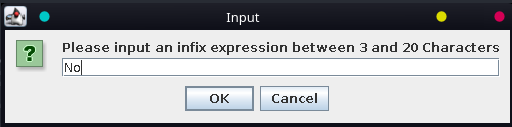
\includegraphics{1.png}
		\end{figure}
		\begin{figure}[h!]
		\centering
		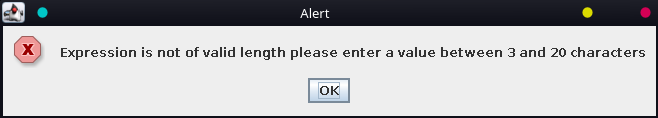
\includegraphics{2.png}
		\end{figure}
		\begin{figure}[h!]
			\centering
			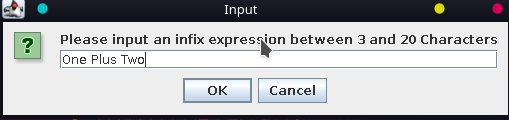
\includegraphics{3.png}
		\end{figure}
		\begin{figure}[h!]
			\centering
			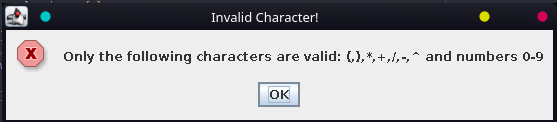
\includegraphics{5.png}
		\end{figure}
		\begin{figure}[h!]
			\centering
			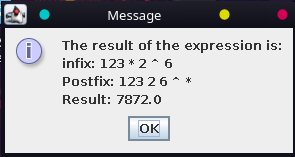
\includegraphics{4.png}
		\end{figure}

	\bibliographystyle{agsm}
	\bibliography{references}
\end{document}
